% This must be in the first 5 lines to tell arXiv to use pdfLaTeX, which is strongly recommended.
\pdfoutput=1
% In particular, the hyperref package requires pdfLaTeX in order to break URLs across lines.
\pdfminorversion=7
\pdfobjcompresslevel=3
\pdfcompresslevel=9


\documentclass[11pt]{article}

% Change "review" to "final" to generate the final (sometimes called camera-ready) version.
\usepackage{acl}

% Standard package includes
\usepackage{times}
\usepackage{latexsym}

% For proper rendering and hyphenation of words containing Latin characters (including in bib files)
\usepackage[T1]{fontenc}

% This assumes your files are encoded as UTF8
\usepackage[utf8]{inputenc}

\usepackage{amsmath}

% This is not strictly necessary, and may be commented out,
% but it will improve the layout of the manuscript,
% and will typically save some space.
\usepackage{microtype}

% This is also not strictly necessary, and may be commented out.
% However, it will improve the aesthetics of text in
% the typewriter font.
\usepackage{inconsolata}

%Including images in your LaTeX document requires adding
%additional package(s)
\usepackage{graphicx}

\title{Etude du meilleur classifieur pour le DEFT de 2009}

\author{
  \text{MANSERI Kéhina\textsuperscript{(1)(2)}}
  \text{SIRVEN-VIENOT Alix\textsuperscript{(1)(2)}}
  \text{VAN-DEN-ZANDE Débora\textsuperscript{(1)(3)}}
\\
\\
  \textsuperscript{(1)}Université Paris Nanterre
  \textsuperscript{(2)}Parcours Recherche et Développement
  \textsuperscript{(3)}Parcours Pro
\\
\\
    \small {
    manserikehina@gmail.com, alix.vienot@gmail.com, vdzdebora@gmail.com
    }
\\
}

\begin{document}
\maketitle
\begin{abstract}
Coucou bouh abstract ! On va expliquer pleins de trucs mais pour l'instant on sait pas ce qu'on fait donc no lol.

Si on veut citer le texte on peut faire comme ça \cite{forest2009variation} et je trouve ça très stylé.

\end{abstract}

\section{Introduction}
Vous pouvez retrouver notre travail sur notre GitHub\footnote{\url{https://github.com/KehinaleK/deft09/tree/main}} pour accéder à l'entièreté de notre code.

Dans cet article, nous présentons nos résultats pour la recherche 

\section{Présentation des données}

\begin{figure}[h]
  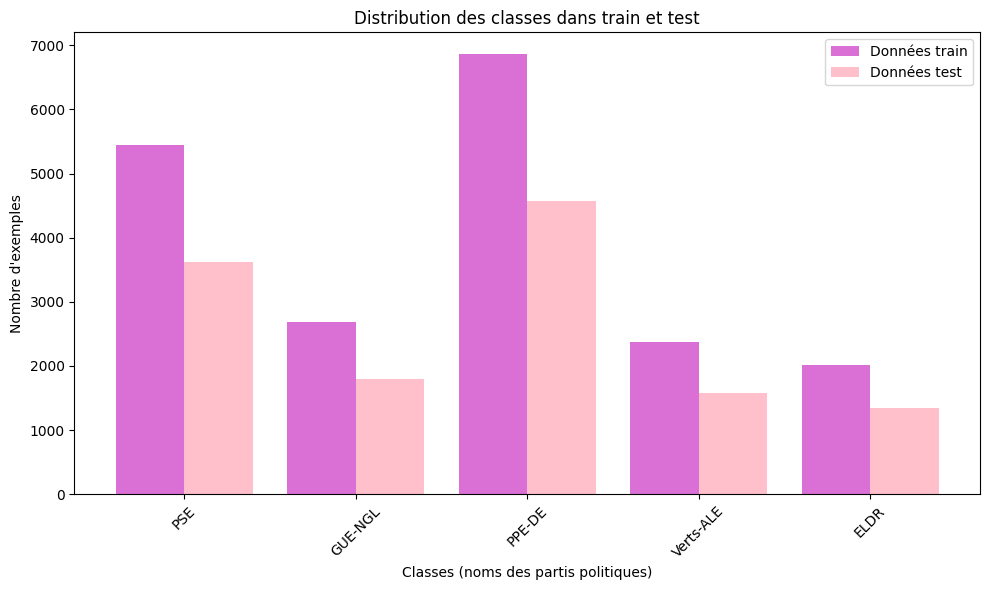
\includegraphics[width=\columnwidth]{latex/graphique_avant.png}
  \caption{Répartition des classes \textbf{avant} nettoyage et rééquilibrage du split}
  \label{fig:graph_avant} % pareil pour citer Figure~\ref{fig:graph_avant}
\end{figure}

\begin{figure}[h]
  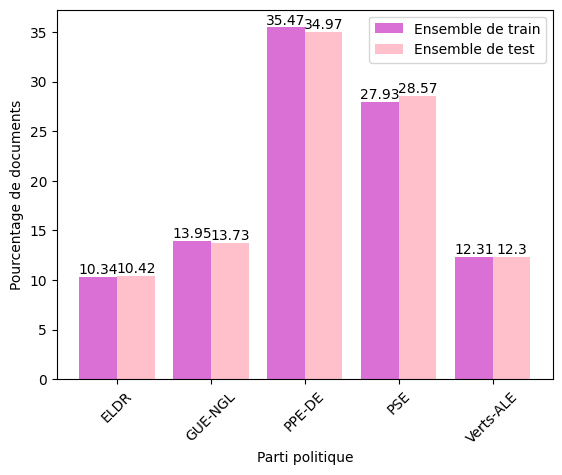
\includegraphics[width=\columnwidth]{latex/graphique_apres.png}
  \caption{Répartition des classes \textbf{après} nettoyage et rééquilibrage du split}
  \label{fig:graph_apres} % Figure~\ref{fig:graph_apres}
\end{figure}

\subsection{Extraction des données}

\subsection{Suppression des doublons}

\subsection{Distribution des classes}
Voir les Figures~\ref{fig:graph_avant} et~\ref{fig:graph_apres} pour une comparaison.

\section{Pré-traitement des données}

\subsection{Normalisation des données}

\subsection{Vectorisation des données}

\section{Comparaison des modèles}
Nous avons décidé de tester plusieurs modèles qui ont des types de classifications différentes (cf. Tableau~\ref{tab:classifieurs_types}).

\begin{table}[h]
    \centering
    \begin{tabular}{|l|l|}
        \hline
        \textbf{Nom du Classifieur}        & \textbf{Type} \\ \hline
        LinearSVC                         & Linéaire      \\ \hline
        RandomForestClassifier            & Ensemble      \\ \hline
        KNeighborsClassifier              & Non-linéaire  \\ \hline
        PassiveAggressiveClassifier       & Linéaire      \\ \hline
        MultinomialNB                     & Probabiliste  \\ \hline
        ComplementNB                      & Probabiliste  \\ \hline
        SVC                               & Non-linéaire  \\ \hline
        RidgeClassifier                   & Linéaire      \\ \hline
        LGBMClassifier                    & Ensemble      \\ \hline
        LogisticRegression                & Linéaire      \\ \hline
        SGDClassifier                     & Linéaire      \\ \hline
    \end{tabular}
    \caption{Liste des classifieurs et leur type.}
    \label{tab:classifieurs_types} % ça c'est pour le citer après ! Tableau~\ref{tab:classifieurs_types}
\end{table}

\subsection{Choix des algorithmes}
Pour notre étude, nous avons choisi de tester un large éventail de modèles, incluant des approches linéaires, probabilistes, non-linéaires et des ensembles. Bien que nous savions qu'il était possible de concentrer nos efforts sur un seul type d'algorithme, nous avons profité du temps disponible pour explorer différents classifieurs. Cette approche nous permet non seulement de comparer les performances des algorithmes, mais aussi de valider notre hypothèse concernant l'impact des déséquilibres de classes dans nos données.

Nos données étant extrêmement déséquilibrées, nous anticipons que les modèles linéaires auront des performances limitées, car ils sont souvent moins adaptés à ce type de scénario. En revanche, les modèles probabilistes, tels que MultinomialNB et ComplementNB, sont particulièrement bien adaptés aux jeux de données déséquilibrés grâce à leur capacité à estimer directement des probabilités de classes.

Cette exploration nous permettra de retenir les trois meilleurs algorithmes à l'issue de nos tests. Ces résultats serviront également à justifier nos choix méthodologiques et à appuyer notre intuition selon laquelle les modèles probabilistes et les modèles utilisant des techniques d'ensemble (comme Random Forest ou LGBMClassifier) seront mieux adaptés aux particularités de nos données. En procédant ainsi, nous avons cherché à maximiser la robustesse de notre analyse tout en assurant une base solide pour nos conclusions.

\subsection{Organisation de la comparaison}

\section{Stratégies d'amélioriation}


\section{Évaluation des modèles}

\subsection{Métriques d'évaluation}
\begin{table}[ht]
    \centering
    \begin{tabular}{|l|c|c|c|}
        \hline
        \textbf{Algorithme} & \textbf{Précision} & \textbf{Rappel} & \textbf{F1-score} \\ \hline
        Logistic Regression & 0.85               & 0.82            & 0.83              \\ \hline
        Random Forest       & 0.88               & 0.85            & 0.86              \\ \hline
        SVM                 & 0.87               & 0.84            & 0.85              \\ \hline
    \end{tabular}
    \caption{Résultats des algorithmes sur les métriques de classification.}
    \label{tab:resultats_algo}
\end{table}

\subsection{Analyse des résultats}


\section{Conclusion}


\bibliography{custom}
\cite{forest2009variation}

\end{document}